\documentclass[]{article}
\usepackage{lmodern}
\usepackage{amssymb,amsmath}
\usepackage{ifxetex,ifluatex}
\usepackage{fixltx2e} % provides \textsubscript
\ifnum 0\ifxetex 1\fi\ifluatex 1\fi=0 % if pdftex
  \usepackage[T1]{fontenc}
  \usepackage[utf8]{inputenc}
\else % if luatex or xelatex
  \ifxetex
    \usepackage{mathspec}
  \else
    \usepackage{fontspec}
  \fi
  \defaultfontfeatures{Ligatures=TeX,Scale=MatchLowercase}
\fi
% use upquote if available, for straight quotes in verbatim environments
\IfFileExists{upquote.sty}{\usepackage{upquote}}{}
% use microtype if available
\IfFileExists{microtype.sty}{%
\usepackage{microtype}
\UseMicrotypeSet[protrusion]{basicmath} % disable protrusion for tt fonts
}{}
\usepackage[margin=1in]{geometry}
\usepackage{hyperref}
\PassOptionsToPackage{usenames,dvipsnames}{color} % color is loaded by hyperref
\hypersetup{unicode=true,
            pdftitle={CWRU DSCI351-351M-451: HW1},
            pdfauthor={Prof.:Roger French, TA:JiQi Liu, Student:Anish Mitra},
            colorlinks=true,
            linkcolor=Maroon,
            citecolor=Blue,
            urlcolor=blue,
            breaklinks=true}
\urlstyle{same}  % don't use monospace font for urls
\usepackage{color}
\usepackage{fancyvrb}
\newcommand{\VerbBar}{|}
\newcommand{\VERB}{\Verb[commandchars=\\\{\}]}
\DefineVerbatimEnvironment{Highlighting}{Verbatim}{commandchars=\\\{\}}
% Add ',fontsize=\small' for more characters per line
\usepackage{framed}
\definecolor{shadecolor}{RGB}{248,248,248}
\newenvironment{Shaded}{\begin{snugshade}}{\end{snugshade}}
\newcommand{\AlertTok}[1]{\textcolor[rgb]{0.94,0.16,0.16}{#1}}
\newcommand{\AnnotationTok}[1]{\textcolor[rgb]{0.56,0.35,0.01}{\textbf{\textit{#1}}}}
\newcommand{\AttributeTok}[1]{\textcolor[rgb]{0.77,0.63,0.00}{#1}}
\newcommand{\BaseNTok}[1]{\textcolor[rgb]{0.00,0.00,0.81}{#1}}
\newcommand{\BuiltInTok}[1]{#1}
\newcommand{\CharTok}[1]{\textcolor[rgb]{0.31,0.60,0.02}{#1}}
\newcommand{\CommentTok}[1]{\textcolor[rgb]{0.56,0.35,0.01}{\textit{#1}}}
\newcommand{\CommentVarTok}[1]{\textcolor[rgb]{0.56,0.35,0.01}{\textbf{\textit{#1}}}}
\newcommand{\ConstantTok}[1]{\textcolor[rgb]{0.00,0.00,0.00}{#1}}
\newcommand{\ControlFlowTok}[1]{\textcolor[rgb]{0.13,0.29,0.53}{\textbf{#1}}}
\newcommand{\DataTypeTok}[1]{\textcolor[rgb]{0.13,0.29,0.53}{#1}}
\newcommand{\DecValTok}[1]{\textcolor[rgb]{0.00,0.00,0.81}{#1}}
\newcommand{\DocumentationTok}[1]{\textcolor[rgb]{0.56,0.35,0.01}{\textbf{\textit{#1}}}}
\newcommand{\ErrorTok}[1]{\textcolor[rgb]{0.64,0.00,0.00}{\textbf{#1}}}
\newcommand{\ExtensionTok}[1]{#1}
\newcommand{\FloatTok}[1]{\textcolor[rgb]{0.00,0.00,0.81}{#1}}
\newcommand{\FunctionTok}[1]{\textcolor[rgb]{0.00,0.00,0.00}{#1}}
\newcommand{\ImportTok}[1]{#1}
\newcommand{\InformationTok}[1]{\textcolor[rgb]{0.56,0.35,0.01}{\textbf{\textit{#1}}}}
\newcommand{\KeywordTok}[1]{\textcolor[rgb]{0.13,0.29,0.53}{\textbf{#1}}}
\newcommand{\NormalTok}[1]{#1}
\newcommand{\OperatorTok}[1]{\textcolor[rgb]{0.81,0.36,0.00}{\textbf{#1}}}
\newcommand{\OtherTok}[1]{\textcolor[rgb]{0.56,0.35,0.01}{#1}}
\newcommand{\PreprocessorTok}[1]{\textcolor[rgb]{0.56,0.35,0.01}{\textit{#1}}}
\newcommand{\RegionMarkerTok}[1]{#1}
\newcommand{\SpecialCharTok}[1]{\textcolor[rgb]{0.00,0.00,0.00}{#1}}
\newcommand{\SpecialStringTok}[1]{\textcolor[rgb]{0.31,0.60,0.02}{#1}}
\newcommand{\StringTok}[1]{\textcolor[rgb]{0.31,0.60,0.02}{#1}}
\newcommand{\VariableTok}[1]{\textcolor[rgb]{0.00,0.00,0.00}{#1}}
\newcommand{\VerbatimStringTok}[1]{\textcolor[rgb]{0.31,0.60,0.02}{#1}}
\newcommand{\WarningTok}[1]{\textcolor[rgb]{0.56,0.35,0.01}{\textbf{\textit{#1}}}}
\usepackage{graphicx,grffile}
\makeatletter
\def\maxwidth{\ifdim\Gin@nat@width>\linewidth\linewidth\else\Gin@nat@width\fi}
\def\maxheight{\ifdim\Gin@nat@height>\textheight\textheight\else\Gin@nat@height\fi}
\makeatother
% Scale images if necessary, so that they will not overflow the page
% margins by default, and it is still possible to overwrite the defaults
% using explicit options in \includegraphics[width, height, ...]{}
\setkeys{Gin}{width=\maxwidth,height=\maxheight,keepaspectratio}
\IfFileExists{parskip.sty}{%
\usepackage{parskip}
}{% else
\setlength{\parindent}{0pt}
\setlength{\parskip}{6pt plus 2pt minus 1pt}
}
\setlength{\emergencystretch}{3em}  % prevent overfull lines
\providecommand{\tightlist}{%
  \setlength{\itemsep}{0pt}\setlength{\parskip}{0pt}}
\setcounter{secnumdepth}{5}
% Redefines (sub)paragraphs to behave more like sections
\ifx\paragraph\undefined\else
\let\oldparagraph\paragraph
\renewcommand{\paragraph}[1]{\oldparagraph{#1}\mbox{}}
\fi
\ifx\subparagraph\undefined\else
\let\oldsubparagraph\subparagraph
\renewcommand{\subparagraph}[1]{\oldsubparagraph{#1}\mbox{}}
\fi

%%% Use protect on footnotes to avoid problems with footnotes in titles
\let\rmarkdownfootnote\footnote%
\def\footnote{\protect\rmarkdownfootnote}

%%% Change title format to be more compact
\usepackage{titling}

% Create subtitle command for use in maketitle
\newcommand{\subtitle}[1]{
  \posttitle{
    \begin{center}\large#1\end{center}
    }
}

\setlength{\droptitle}{-2em}

  \title{CWRU DSCI351-351M-451: HW1}
    \pretitle{\vspace{\droptitle}\centering\huge}
  \posttitle{\par}
    \author{Prof.:Roger French, TA:JiQi Liu, Student:Anish Mitra}
    \preauthor{\centering\large\emph}
  \postauthor{\par}
      \predate{\centering\large\emph}
  \postdate{\par}
    \date{August 30, 2017, Due Tuesday September 4th, before class}


\begin{document}
\maketitle

{
\hypersetup{linkcolor=black}
\setcounter{tocdepth}{2}
\tableofcontents
}
\setcounter{section}{1} \setcounter{subsection}{0}

\hypertarget{so-by-now-i-believe-everyone-has}{%
\subsection{So by now I believe everyone
has}\label{so-by-now-i-believe-everyone-has}}

\hypertarget{logged-into-your-ods-vdi-or-your-vuvlab-vdi.}{%
\subsubsection{Logged into your ODS VDI, or your VUVlab
VDI.}\label{logged-into-your-ods-vdi-or-your-vuvlab-vdi.}}

\begin{verbatim}
- If not send the help@case.edu helpdesk an email, 
  - directed to CSE-IT, saying you are in DSCI351/351M/451 
  - and should have access to the ODS VDI, 
  - that you use Citrix REceiver to connect to.
\end{verbatim}

\hypertarget{your-h-drive-is-big-enough}{%
\subsubsection{Your H: drive is big
enough}\label{your-h-drive-is-big-enough}}

\begin{itemize}
\tightlist
\item
  so that you can Git clone your personal fork of the Prof repo,
\item
  from Bitbucket down to \texttt{H:\textbackslash{}Git\textbackslash{}}
  folder.
\end{itemize}

\hypertarget{youll-notice-in-hw1}{%
\subsubsection{You'll notice in HW1}\label{youll-notice-in-hw1}}

\begin{itemize}
\tightlist
\item
  That there is an initial read Leek's structure of a data analysis.\\
\item
  This all students should do.
\end{itemize}

\hypertarget{ask-questions-in-cwru-dsci-slack-channel-for-dsci351-351m-451}{%
\subsubsection{Ask Questions in CWRU-DSCI Slack Channel for
DSCI351-351M-451}\label{ask-questions-in-cwru-dsci-slack-channel-for-dsci351-351m-451}}

\begin{itemize}
\tightlist
\item
  This is the easier way to ask and answer questions
\item
  You can use @JiQi Liu and @Roger French

  \begin{itemize}
  \tightlist
  \item
    To direct a question to us
  \item
    But anyone can answer the questions
  \end{itemize}
\end{itemize}

\hypertarget{m-and-451-students}{%
\subsection{351, 351M and 451 students}\label{m-and-451-students}}

\begin{itemize}
\tightlist
\item
  will both do the last part of the homework,

  \begin{itemize}
  \tightlist
  \item
    where you are doing some R coding,
  \item
    inside the R code blocks of the Rmd file
  \item
    (between the \(```{r}\) and the \(```\) that closes the R code block
    in the Rmd file.
  \end{itemize}
\end{itemize}

\hypertarget{and-451-students}{%
\subsection{And 451 students}\label{and-451-students}}

\begin{itemize}
\tightlist
\item
  will start writing about what they are considering for their Semester
  Project.

  \begin{itemize}
  \tightlist
  \item
    Read about the 451 Semester Project in
    1-assignments\textgreater{}SemProj-451\textgreater{}1808-451-SemProj-Overview.pdf
  \end{itemize}
\item
  Your SemProj will have 3 in-class report outs on progress, and a final
  full report.
\item
  It should ideally be related to your thesis research,

  \begin{itemize}
  \tightlist
  \item
    and be a data analysis project that will help advance your
    research.\\
  \end{itemize}
\item
  We will be defining and refining what you will do your Semester
  Project on,

  \begin{itemize}
  \tightlist
  \item
    in the next few weeks.
  \end{itemize}
\end{itemize}

\hypertarget{here-are-answers-to-a-few-questions-we-usually-get-about-hw1}{%
\subsection{Here are answers to a few questions we usually get about
HW1}\label{here-are-answers-to-a-few-questions-we-usually-get-about-hw1}}

A. ``I am having trouble converting the Rmd file containing homework 1
into a PDF. I was able to save it as a .txt file--is it okay if I submit
that instead of a PDF?''

Once you have made a *.Rmd file, you compile it to make the pdf, by
hitting the Knit button at the top of the Rstudio text editor, or you
can click on the Knit button to choose Knit to PDF from the choices. You
can also use the keyboard shortcut Cntrl+Shift+K. (You can find lots of
keyboard shortcuts help with Alt+Shift+K).

And if you open the homework 1 Rmd file named
``1808-351-351M-451-hw1-NAME.Rmd'' and change NAME to your own name.
Then you can immediately compile that Rmd file to make the pdf. This way
you'll know that its not some error in what you have added to the file's
text. Compiling to pdf, uses the LaTeX publishing distribution on your
VDI. So if you are trying this on your own personal computer, it won't
work, since you probably don't have a LaTeX distribution, such as MikTeX
(for windows), MacTeX (for Macs), or TexLive for Linux, installed, so
can't produce a LaTeX pdf output.

B. ``I was also wondering where we are supposed to submit our homework
assignments. Are we supposed to upload them onto BitBucket?''

You will upload your *.Rmd file (so we can see your coding style and
commenting), and your compiled Pdf file to our Canvas Assignment page in
canvas.case.edu for the DSCI351-351M-451 class.

\hypertarget{read-the-leek-handout}{%
\subsection{Read the LEEK handout}\label{read-the-leek-handout}}

\begin{itemize}
\tightlist
\item
  in ./readings/1503LeekDataAnalyticStyle-outline.txt
\item
  This is located in
  ./class/Leek/Leek-ADataAnalysisStructureAndOrganizing.pdf
\item
  and look at Leek's book in ./readings/Texts/Leek-DataAnalyticStyle.pdf
\end{itemize}

\hypertarget{on-organizing-a-data-analysis}{%
\subsubsection{On organizing a data
analysis}\label{on-organizing-a-data-analysis}}

\begin{itemize}
\tightlist
\item
  Jeff Leek is a biostatistician
\item
  At Johns Hopkins School of Public Health
\end{itemize}

\hypertarget{steps-in-a-data-analysis}{%
\subsubsection{Steps in a data
analysis}\label{steps-in-a-data-analysis}}

\begin{itemize}
\tightlist
\item
  Define the question
\item
  Define the ideal data set
\item
  Determine what data you can access
\item
  Obtain the data
\item
  Clean the data
\item
  Exploratory data analysis
\item
  Statistical prediction/modeling
\item
  Interpret results
\item
  Challenge results
\item
  Synthesize/write up results
\item
  Create reproducible code
\end{itemize}

\hypertarget{dsci-451-hw1-assignment}{%
\subsection{DSCI 451 HW1 Assignment}\label{dsci-451-hw1-assignment}}

\begin{itemize}
\tightlist
\item
  Make an separate Rmarkdown file (*.Rmd) discussing your Semester
  Project
\item
  Which you compile to produce a pdf report
\item
  About a data analysis question of interest to you

  \begin{itemize}
  \tightlist
  \item
    Use figures, sections, math equations and hyperlinks
  \item
    Author, License, Version number, Changelog
  \end{itemize}
\item
  Submit the .Rmd file and the pdf on Canvas
\end{itemize}

\hypertarget{for-dsci451-grad-students}{%
\subsubsection{For DSCI451 Grad
Students}\label{for-dsci451-grad-students}}

\begin{itemize}
\tightlist
\item
  This Rmd will be an initial proposal

  \begin{itemize}
  \tightlist
  \item
    Of your semester data science project
  \end{itemize}
\item
  Explain background of questin
\item
  Experiments or approaches
\item
  Data types and characterisitics.
\item
  Use figures, sections, math equations and hyperlinks
\end{itemize}

\hypertarget{dsci-351351m451}{%
\subsection{DSCI 351/351M/451}\label{dsci-351351m451}}

\begin{itemize}
\tightlist
\item
  Enter all work into this rmd file
\item
  Make sure it compiles and submit both the rmd and pdf
\item
  Rmd documents run code in block segments

  \begin{itemize}
  \tightlist
  \item
    defined and closed by \(```\) with an option to provide parameters
  \end{itemize}
\end{itemize}

\begin{Shaded}
\begin{Highlighting}[]
\KeywordTok{print}\NormalTok{(}\StringTok{'hello world'}\NormalTok{)}
\end{Highlighting}
\end{Shaded}

\begin{verbatim}
## [1] "hello world"
\end{verbatim}

\begin{itemize}
\tightlist
\item
  Answer all questions in below in the provided code blocks
\end{itemize}

\hypertarget{basic-r-operations}{%
\subsubsection{Basic R operations}\label{basic-r-operations}}

\begin{itemize}
\tightlist
\item
  Show an example of addition, subtraction, multiplication, division,
  and an exponential below
\end{itemize}

\begin{Shaded}
\begin{Highlighting}[]
\CommentTok{#Example of addition}
\KeywordTok{print}\NormalTok{(}\StringTok{"Addition"}\NormalTok{)}
\end{Highlighting}
\end{Shaded}

\begin{verbatim}
## [1] "Addition"
\end{verbatim}

\begin{Shaded}
\begin{Highlighting}[]
\NormalTok{x <-}\StringTok{ }\DecValTok{1} \OperatorTok{+}\StringTok{ }\DecValTok{1}
\NormalTok{x}
\end{Highlighting}
\end{Shaded}

\begin{verbatim}
## [1] 2
\end{verbatim}

\begin{Shaded}
\begin{Highlighting}[]
\CommentTok{#Example of subtraction}
\KeywordTok{print}\NormalTok{(}\StringTok{"Subtraction"}\NormalTok{)}
\end{Highlighting}
\end{Shaded}

\begin{verbatim}
## [1] "Subtraction"
\end{verbatim}

\begin{Shaded}
\begin{Highlighting}[]
\NormalTok{y <-}\StringTok{ }\DecValTok{2} \OperatorTok{-}\StringTok{ }\DecValTok{2}
\NormalTok{y}
\end{Highlighting}
\end{Shaded}

\begin{verbatim}
## [1] 0
\end{verbatim}

\begin{Shaded}
\begin{Highlighting}[]
\CommentTok{#Example of multiplication}
\KeywordTok{print}\NormalTok{(}\StringTok{"Multiplication"}\NormalTok{)}
\end{Highlighting}
\end{Shaded}

\begin{verbatim}
## [1] "Multiplication"
\end{verbatim}

\begin{Shaded}
\begin{Highlighting}[]
\NormalTok{z <-}\StringTok{ }\DecValTok{2} \OperatorTok{*}\StringTok{ }\DecValTok{2}
\NormalTok{z}
\end{Highlighting}
\end{Shaded}

\begin{verbatim}
## [1] 4
\end{verbatim}

\begin{Shaded}
\begin{Highlighting}[]
\CommentTok{#Example of division}
\KeywordTok{print}\NormalTok{(}\StringTok{"Division"}\NormalTok{)}
\end{Highlighting}
\end{Shaded}

\begin{verbatim}
## [1] "Division"
\end{verbatim}

\begin{Shaded}
\begin{Highlighting}[]
\NormalTok{a <-}\StringTok{ }\DecValTok{2} \OperatorTok{/}\StringTok{ }\DecValTok{2}
\NormalTok{a}
\end{Highlighting}
\end{Shaded}

\begin{verbatim}
## [1] 1
\end{verbatim}

\begin{Shaded}
\begin{Highlighting}[]
\CommentTok{#Example of an exponential}
\KeywordTok{print}\NormalTok{(}\StringTok{"Exponential"}\NormalTok{)}
\end{Highlighting}
\end{Shaded}

\begin{verbatim}
## [1] "Exponential"
\end{verbatim}

\begin{Shaded}
\begin{Highlighting}[]
\NormalTok{b =}\StringTok{ }\DecValTok{2}\OperatorTok{^}\DecValTok{3}
\NormalTok{b}
\end{Highlighting}
\end{Shaded}

\begin{verbatim}
## [1] 8
\end{verbatim}

\hypertarget{working-with-data-frames}{%
\subsubsection{Working with data
frames}\label{working-with-data-frames}}

\begin{itemize}
\tightlist
\item
  Data frames are an important data format in R
\item
  Example data can be loaded from base R
\item
  Run the code below to load the iris dataset into your environment
\item
  This data set will be used for the later problems
\end{itemize}

\begin{Shaded}
\begin{Highlighting}[]
\KeywordTok{data}\NormalTok{(}\StringTok{"iris"}\NormalTok{)}
\KeywordTok{head}\NormalTok{(iris)}
\end{Highlighting}
\end{Shaded}

\begin{verbatim}
##   Sepal.Length Sepal.Width Petal.Length Petal.Width Species
## 1          5.1         3.5          1.4         0.2  setosa
## 2          4.9         3.0          1.4         0.2  setosa
## 3          4.7         3.2          1.3         0.2  setosa
## 4          4.6         3.1          1.5         0.2  setosa
## 5          5.0         3.6          1.4         0.2  setosa
## 6          5.4         3.9          1.7         0.4  setosa
\end{verbatim}

\begin{itemize}
\tightlist
\item
  Give the class of each of the columns in the iris data set
\item
  Explain in code comments what is a factor and how it differs from a
  character
\end{itemize}

\begin{Shaded}
\begin{Highlighting}[]
\NormalTok{x <-}\StringTok{ }\KeywordTok{lapply}\NormalTok{(iris, class)}
\NormalTok{x}
\end{Highlighting}
\end{Shaded}

\begin{verbatim}
## $Sepal.Length
## [1] "numeric"
## 
## $Sepal.Width
## [1] "numeric"
## 
## $Petal.Length
## [1] "numeric"
## 
## $Petal.Width
## [1] "numeric"
## 
## $Species
## [1] "factor"
\end{verbatim}

\begin{Shaded}
\begin{Highlighting}[]
\CommentTok{#The difference is that a factor is a categorical variable whereas a factor #variable is not.This basically means that factors have character levels. These #levels categorise the data. Consequentially, factors have a different number #of data values which it can distinguish between.}
\end{Highlighting}
\end{Shaded}

\begin{itemize}
\tightlist
\item
  Use the table() function to determine how many species there are

  \begin{itemize}
  \tightlist
  \item
    and how many observation each one has (Species column in the data
    frame)
  \end{itemize}
\end{itemize}

\begin{Shaded}
\begin{Highlighting}[]
\KeywordTok{class}\NormalTok{(iris)}
\end{Highlighting}
\end{Shaded}

\begin{verbatim}
## [1] "data.frame"
\end{verbatim}

\begin{Shaded}
\begin{Highlighting}[]
\KeywordTok{table}\NormalTok{(iris[}\DecValTok{5}\NormalTok{])}
\end{Highlighting}
\end{Shaded}

\begin{verbatim}
## 
##     setosa versicolor  virginica 
##         50         50         50
\end{verbatim}

\begin{itemize}
\tightlist
\item
  Use the subset() function create a new data frame of only versicolor
  flower data
\end{itemize}

\begin{Shaded}
\begin{Highlighting}[]
\NormalTok{versicolor <-}\StringTok{ }\NormalTok{iris[}\DecValTok{5}\NormalTok{]}
\NormalTok{versicolordataframe <-}\StringTok{ }\KeywordTok{subset.data.frame}\NormalTok{(iris, versicolor }\OperatorTok{==}\StringTok{ "versicolor"}\NormalTok{)}
\NormalTok{versicolordataframe}
\end{Highlighting}
\end{Shaded}

\begin{verbatim}
##     Sepal.Length Sepal.Width Petal.Length Petal.Width    Species
## 51           7.0         3.2          4.7         1.4 versicolor
## 52           6.4         3.2          4.5         1.5 versicolor
## 53           6.9         3.1          4.9         1.5 versicolor
## 54           5.5         2.3          4.0         1.3 versicolor
## 55           6.5         2.8          4.6         1.5 versicolor
## 56           5.7         2.8          4.5         1.3 versicolor
## 57           6.3         3.3          4.7         1.6 versicolor
## 58           4.9         2.4          3.3         1.0 versicolor
## 59           6.6         2.9          4.6         1.3 versicolor
## 60           5.2         2.7          3.9         1.4 versicolor
## 61           5.0         2.0          3.5         1.0 versicolor
## 62           5.9         3.0          4.2         1.5 versicolor
## 63           6.0         2.2          4.0         1.0 versicolor
## 64           6.1         2.9          4.7         1.4 versicolor
## 65           5.6         2.9          3.6         1.3 versicolor
## 66           6.7         3.1          4.4         1.4 versicolor
## 67           5.6         3.0          4.5         1.5 versicolor
## 68           5.8         2.7          4.1         1.0 versicolor
## 69           6.2         2.2          4.5         1.5 versicolor
## 70           5.6         2.5          3.9         1.1 versicolor
## 71           5.9         3.2          4.8         1.8 versicolor
## 72           6.1         2.8          4.0         1.3 versicolor
## 73           6.3         2.5          4.9         1.5 versicolor
## 74           6.1         2.8          4.7         1.2 versicolor
## 75           6.4         2.9          4.3         1.3 versicolor
## 76           6.6         3.0          4.4         1.4 versicolor
## 77           6.8         2.8          4.8         1.4 versicolor
## 78           6.7         3.0          5.0         1.7 versicolor
## 79           6.0         2.9          4.5         1.5 versicolor
## 80           5.7         2.6          3.5         1.0 versicolor
## 81           5.5         2.4          3.8         1.1 versicolor
## 82           5.5         2.4          3.7         1.0 versicolor
## 83           5.8         2.7          3.9         1.2 versicolor
## 84           6.0         2.7          5.1         1.6 versicolor
## 85           5.4         3.0          4.5         1.5 versicolor
## 86           6.0         3.4          4.5         1.6 versicolor
## 87           6.7         3.1          4.7         1.5 versicolor
## 88           6.3         2.3          4.4         1.3 versicolor
## 89           5.6         3.0          4.1         1.3 versicolor
## 90           5.5         2.5          4.0         1.3 versicolor
## 91           5.5         2.6          4.4         1.2 versicolor
## 92           6.1         3.0          4.6         1.4 versicolor
## 93           5.8         2.6          4.0         1.2 versicolor
## 94           5.0         2.3          3.3         1.0 versicolor
## 95           5.6         2.7          4.2         1.3 versicolor
## 96           5.7         3.0          4.2         1.2 versicolor
## 97           5.7         2.9          4.2         1.3 versicolor
## 98           6.2         2.9          4.3         1.3 versicolor
## 99           5.1         2.5          3.0         1.1 versicolor
## 100          5.7         2.8          4.1         1.3 versicolor
\end{verbatim}

\begin{itemize}
\tightlist
\item
  Give the mean and median of each of the numeric columns for the
  versicolor data frame
\item
  Why might the mean and median of the entire iris dataset be
  misleading?
\end{itemize}

\begin{Shaded}
\begin{Highlighting}[]
\CommentTok{#Mean and median for sepal length}
\KeywordTok{print}\NormalTok{(}\StringTok{"Mean"}\NormalTok{);}\KeywordTok{lapply}\NormalTok{(versicolordataframe[}\DecValTok{1}\NormalTok{], mean); }\KeywordTok{print}\NormalTok{(}\StringTok{"Median"}\NormalTok{);}\KeywordTok{lapply}\NormalTok{(versicolordataframe[}\DecValTok{1}\NormalTok{], median)}
\end{Highlighting}
\end{Shaded}

\begin{verbatim}
## [1] "Mean"
\end{verbatim}

\begin{verbatim}
## $Sepal.Length
## [1] 5.936
\end{verbatim}

\begin{verbatim}
## [1] "Median"
\end{verbatim}

\begin{verbatim}
## $Sepal.Length
## [1] 5.9
\end{verbatim}

\begin{Shaded}
\begin{Highlighting}[]
\CommentTok{#Mean and median for sepal width}
\KeywordTok{print}\NormalTok{(}\StringTok{"Mean"}\NormalTok{);}\KeywordTok{lapply}\NormalTok{(versicolordataframe[}\DecValTok{2}\NormalTok{], mean); }\KeywordTok{print}\NormalTok{(}\StringTok{"Median"}\NormalTok{);}\KeywordTok{lapply}\NormalTok{(versicolordataframe[}\DecValTok{2}\NormalTok{], median)}
\end{Highlighting}
\end{Shaded}

\begin{verbatim}
## [1] "Mean"
\end{verbatim}

\begin{verbatim}
## $Sepal.Width
## [1] 2.77
\end{verbatim}

\begin{verbatim}
## [1] "Median"
\end{verbatim}

\begin{verbatim}
## $Sepal.Width
## [1] 2.8
\end{verbatim}

\begin{Shaded}
\begin{Highlighting}[]
\CommentTok{#Mean and median for petal length}
\KeywordTok{print}\NormalTok{(}\StringTok{"Mean"}\NormalTok{);}\KeywordTok{lapply}\NormalTok{(versicolordataframe[}\DecValTok{3}\NormalTok{], mean); }\KeywordTok{print}\NormalTok{(}\StringTok{"Median"}\NormalTok{);}\KeywordTok{lapply}\NormalTok{(versicolordataframe[}\DecValTok{3}\NormalTok{], median)}
\end{Highlighting}
\end{Shaded}

\begin{verbatim}
## [1] "Mean"
\end{verbatim}

\begin{verbatim}
## $Petal.Length
## [1] 4.26
\end{verbatim}

\begin{verbatim}
## [1] "Median"
\end{verbatim}

\begin{verbatim}
## $Petal.Length
## [1] 4.35
\end{verbatim}

\begin{Shaded}
\begin{Highlighting}[]
\CommentTok{#Mean and median for petal width}
\KeywordTok{print}\NormalTok{(}\StringTok{"Mean"}\NormalTok{);}\KeywordTok{lapply}\NormalTok{(versicolordataframe[}\DecValTok{4}\NormalTok{], mean); }\KeywordTok{print}\NormalTok{(}\StringTok{"Median"}\NormalTok{);}\KeywordTok{lapply}\NormalTok{(versicolordataframe[}\DecValTok{4}\NormalTok{], median)}
\end{Highlighting}
\end{Shaded}

\begin{verbatim}
## [1] "Mean"
\end{verbatim}

\begin{verbatim}
## $Petal.Width
## [1] 1.326
\end{verbatim}

\begin{verbatim}
## [1] "Median"
\end{verbatim}

\begin{verbatim}
## $Petal.Width
## [1] 1.3
\end{verbatim}

\begin{Shaded}
\begin{Highlighting}[]
\KeywordTok{print}\NormalTok{(}\StringTok{"The mean and median might be misleading since we don't know the standard deviation and therefore we have nothing to compare the mean and median with."}\NormalTok{)}
\end{Highlighting}
\end{Shaded}

\begin{verbatim}
## [1] "The mean and median might be misleading since we don't know the standard deviation and therefore we have nothing to compare the mean and median with."
\end{verbatim}

\begin{Shaded}
\begin{Highlighting}[]
\KeywordTok{print}\NormalTok{(}\StringTok{"The dataset for iris also has three different species so this implies that the mean and median might not be representative. It is better to take the individual species' mean and median first."}\NormalTok{)}
\end{Highlighting}
\end{Shaded}

\begin{verbatim}
## [1] "The dataset for iris also has three different species so this implies that the mean and median might not be representative. It is better to take the individual species' mean and median first."
\end{verbatim}

\hypertarget{modeling-and-plotting}{%
\subsubsection{Modeling and plotting}\label{modeling-and-plotting}}

\begin{itemize}
\tightlist
\item
  Use the lm() and plot() functions to build a simple linear model

  \begin{itemize}
  \tightlist
  \item
    of versicolor petal length as a function of petal width
  \end{itemize}
\item
  What are the dependant and independant variables in this case?
\item
  Add the model to the plot with abline()
\end{itemize}

\begin{Shaded}
\begin{Highlighting}[]
\KeywordTok{print}\NormalTok{(}\StringTok{"The dependent variable is the versicolor petal length and the dependent variable is the petal width"}\NormalTok{)}
\end{Highlighting}
\end{Shaded}

\begin{verbatim}
## [1] "The dependent variable is the versicolor petal length and the dependent variable is the petal width"
\end{verbatim}

\begin{Shaded}
\begin{Highlighting}[]
\NormalTok{petallength <-}\StringTok{ }\NormalTok{versicolordataframe}\OperatorTok{$}\NormalTok{Petal.Length}
\NormalTok{petalwidth <-}\StringTok{ }\NormalTok{versicolordataframe}\OperatorTok{$}\NormalTok{Petal.Width}
\NormalTok{graphofversicolor <-}\StringTok{ }\KeywordTok{plot}\NormalTok{(petalwidth, petallength)}
\NormalTok{graphofversicolor}
\end{Highlighting}
\end{Shaded}

\begin{verbatim}
## NULL
\end{verbatim}

\begin{Shaded}
\begin{Highlighting}[]
\NormalTok{fitofversicolor <-}\StringTok{ }\KeywordTok{lm}\NormalTok{(petallength }\OperatorTok{~}\StringTok{ }\NormalTok{petalwidth, graphofversicolor)}
\KeywordTok{abline}\NormalTok{(fitofversicolor)}
\end{Highlighting}
\end{Shaded}

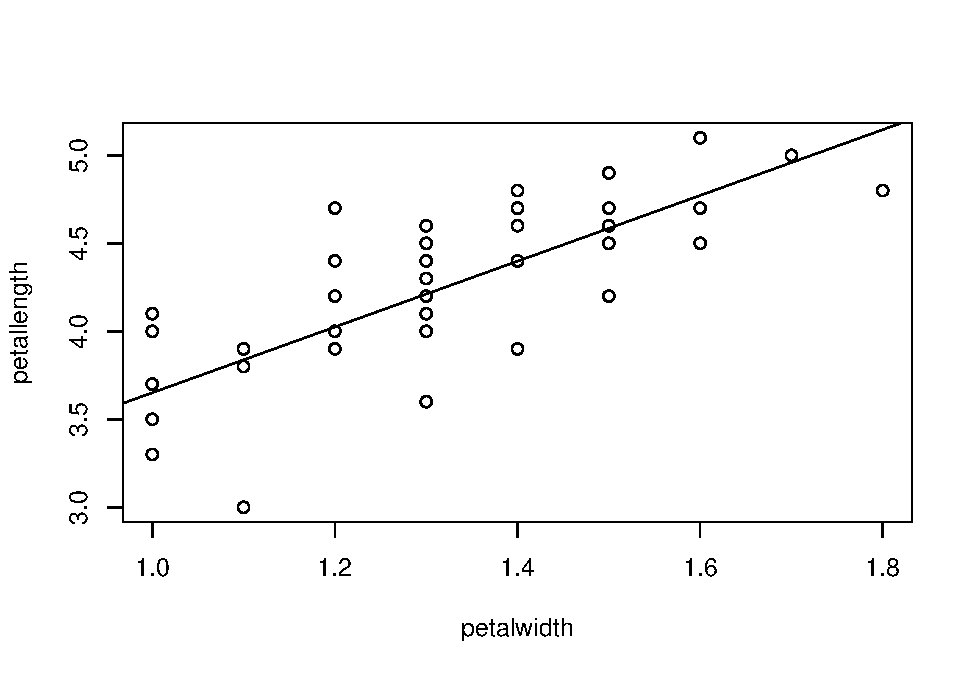
\includegraphics{1808-351-351m451-hw1-Mitra_files/figure-latex/unnamed-chunk-8-1.pdf}

\begin{itemize}
\tightlist
\item
  Print the summary of this model
\end{itemize}

\begin{Shaded}
\begin{Highlighting}[]
\KeywordTok{summary}\NormalTok{(fitofversicolor)}
\end{Highlighting}
\end{Shaded}

\begin{verbatim}
## 
## Call:
## lm(formula = petallength ~ petalwidth, data = graphofversicolor)
## 
## Residuals:
##     Min      1Q  Median      3Q     Max 
## -0.8375 -0.1441 -0.0114  0.1984  0.6755 
## 
## Coefficients:
##             Estimate Std. Error t value Pr(>|t|)    
## (Intercept)   1.7813     0.2838   6.276 9.48e-08 ***
## petalwidth    1.8693     0.2117   8.828 1.27e-11 ***
## ---
## Signif. codes:  0 '***' 0.001 '**' 0.01 '*' 0.05 '.' 0.1 ' ' 1
## 
## Residual standard error: 0.2931 on 48 degrees of freedom
## Multiple R-squared:  0.6188, Adjusted R-squared:  0.6109 
## F-statistic: 77.93 on 1 and 48 DF,  p-value: 1.272e-11
\end{verbatim}

\hypertarget{links}{%
\subsection{Links}\label{links}}

\begin{itemize}
\tightlist
\item
  \url{http://www.r-project.org}
\item
  \url{http://rmarkdown.rstudio.com/}
\end{itemize}

\textless{}!-- \# Keep a complete change log history at bottom of file.
\# Complete Change Log History \# v0.00.00 - 1405-07 - Nick Wheeler made
the blank script \#\#\#\#\#\#\#\#\#\#


\end{document}
